\begin{figure}
    \centering
\minipage{0.32\textwidth}
    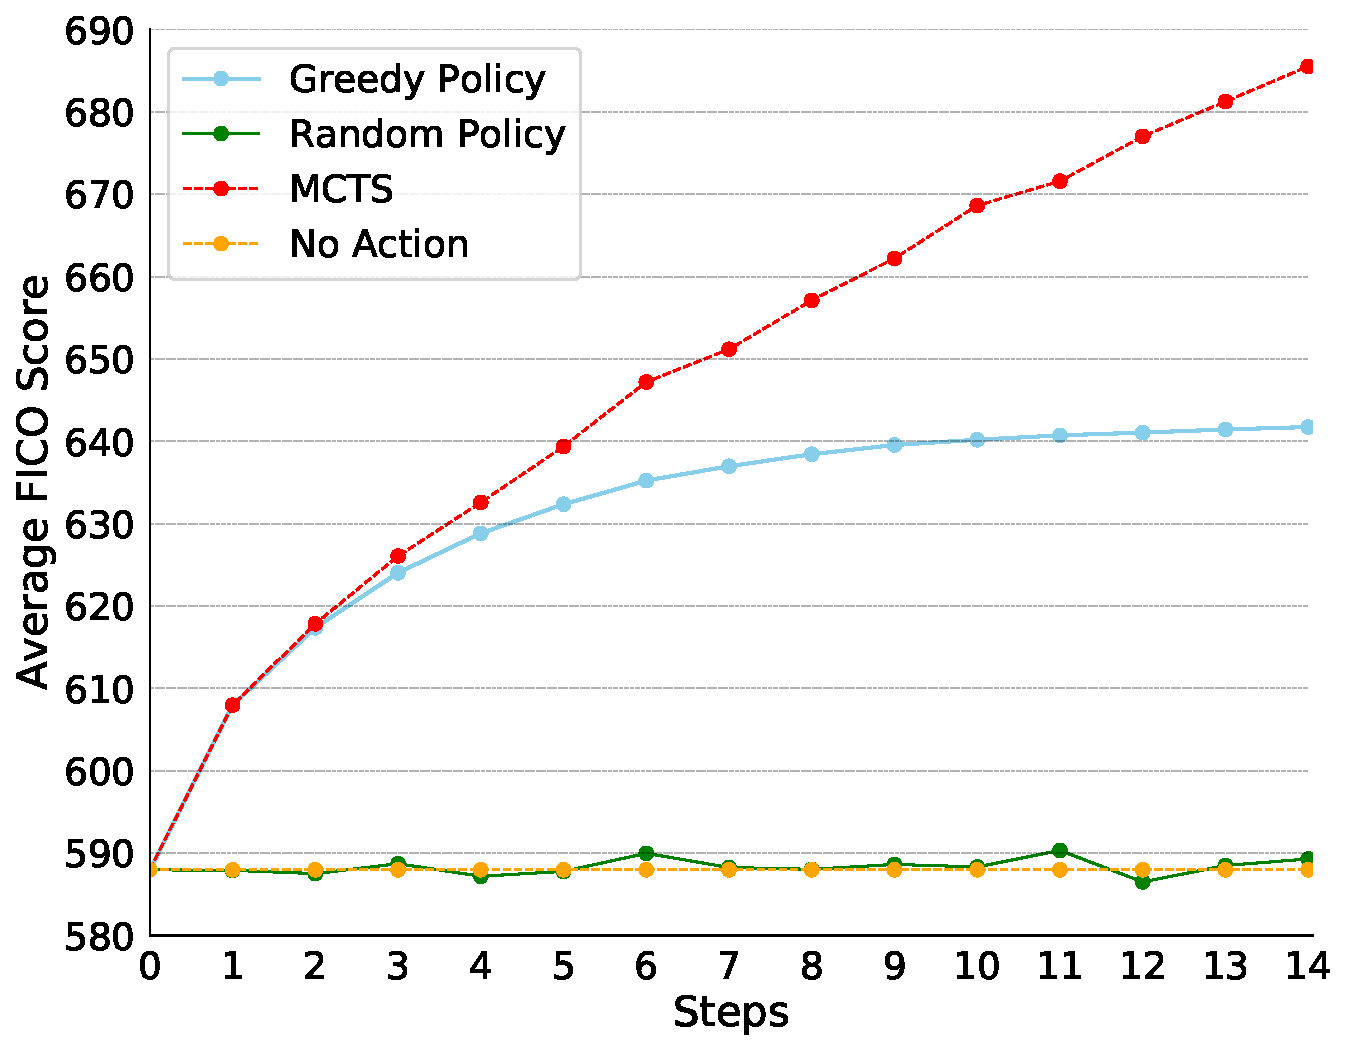
\includegraphics[width=\linewidth]{figures/fixedsimplefico.pdf}
    % \caption{FICO credit scoring averaged over 1000 initial states (higher is better)}
\endminipage\hfill
\minipage{0.32\textwidth}
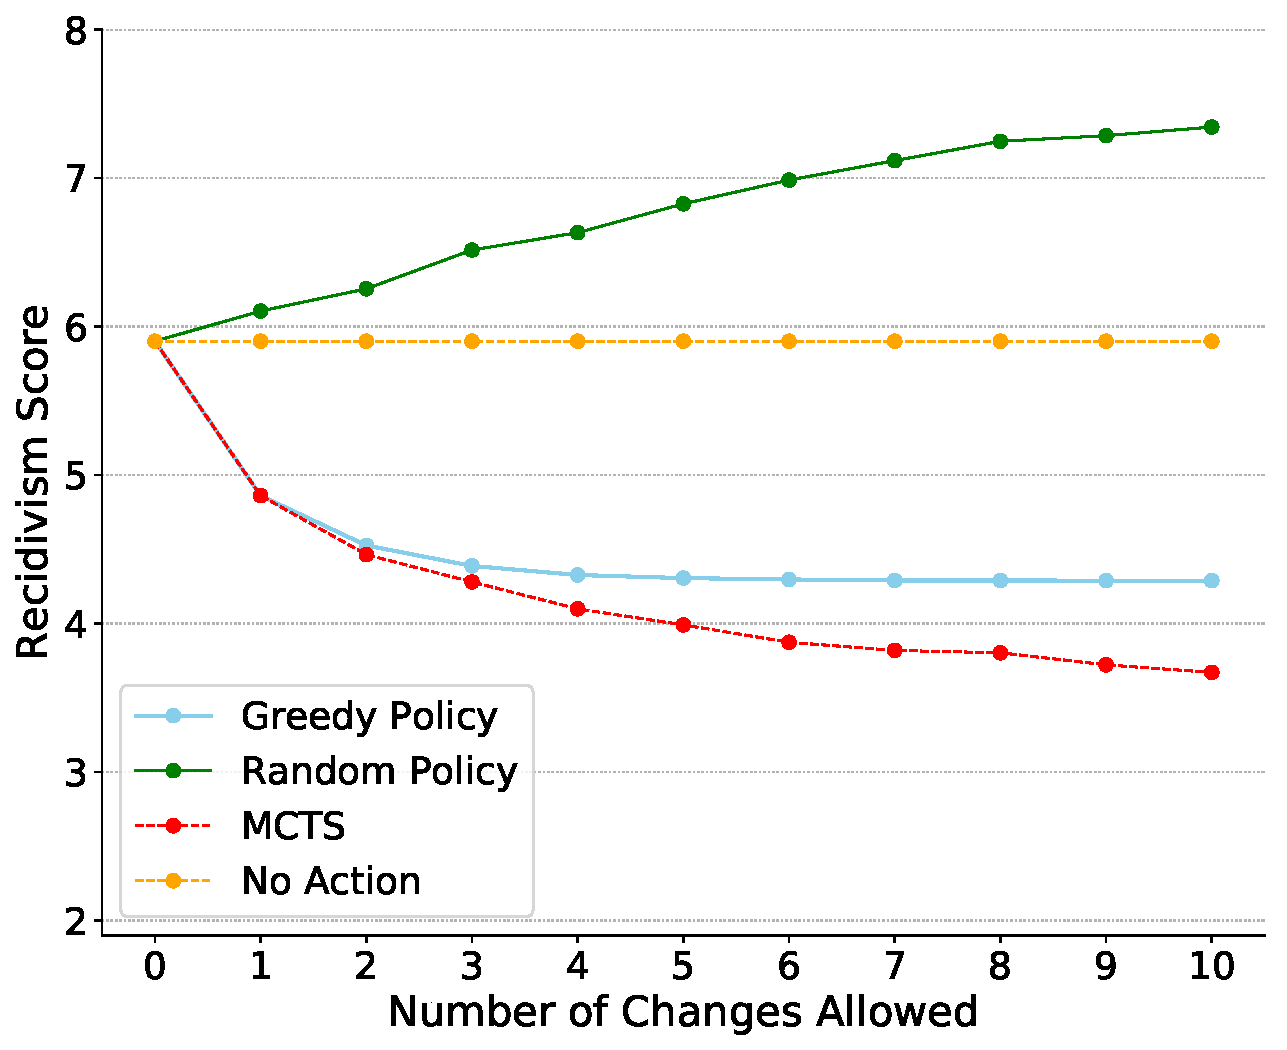
\includegraphics[width=\linewidth]{figures/compas_yi.pdf}
    % \caption{Recidivism prediction including race and gender, averaged over $500$ initial medium/high risk states (lower is better)}
\endminipage\hfill
\minipage{0.32\textwidth}
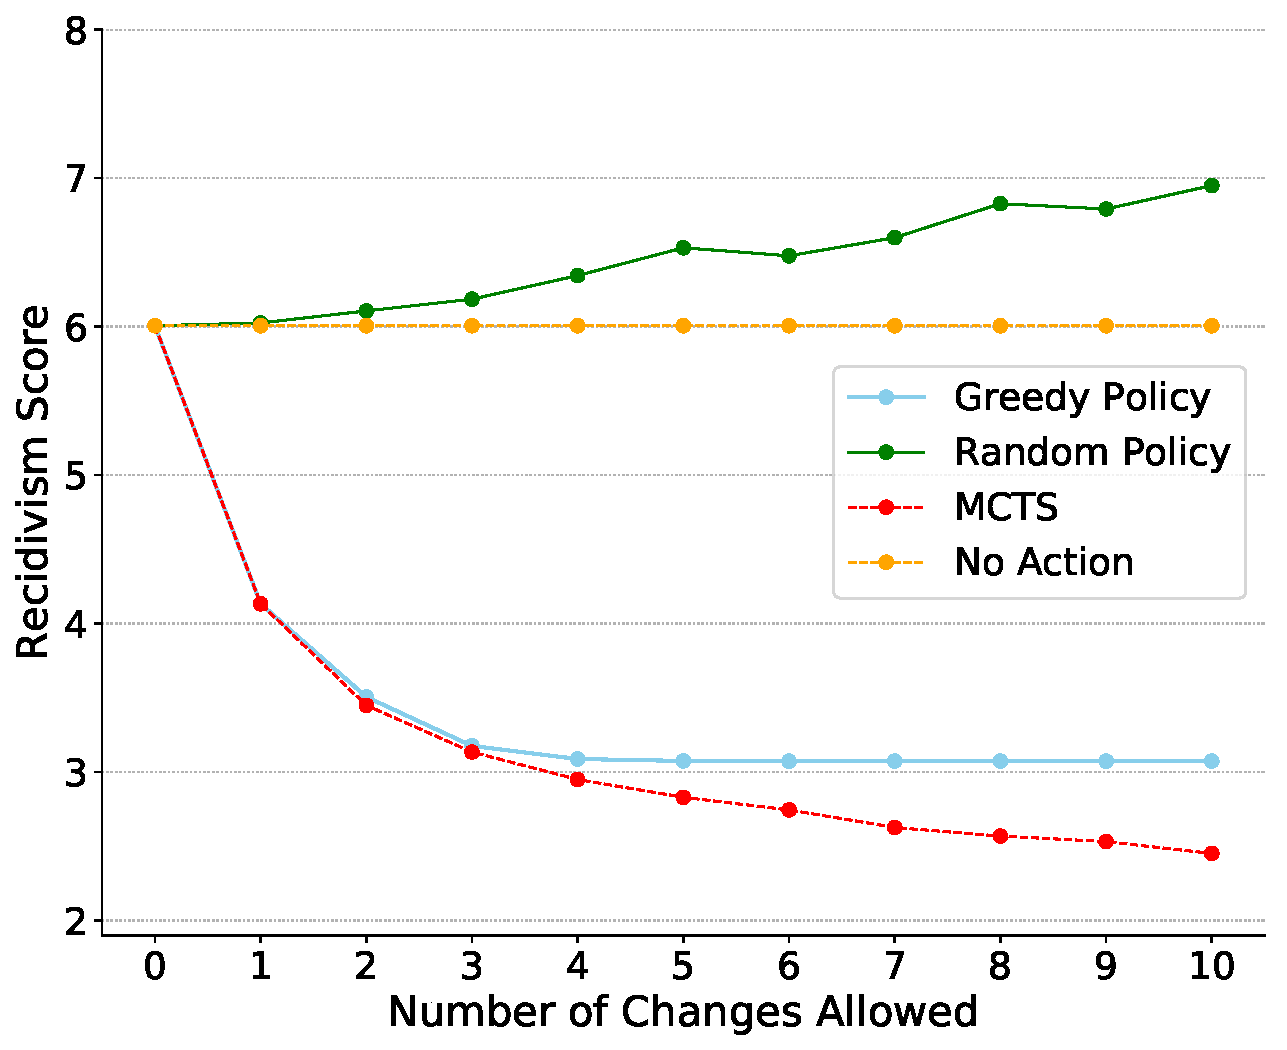
\includegraphics[width=\linewidth]{figures/compas_ni.pdf}
    % \caption{Recidivism prediction excluding race/gender}
\endminipage\hfill
% \minipage{0.24\textwidth}
%     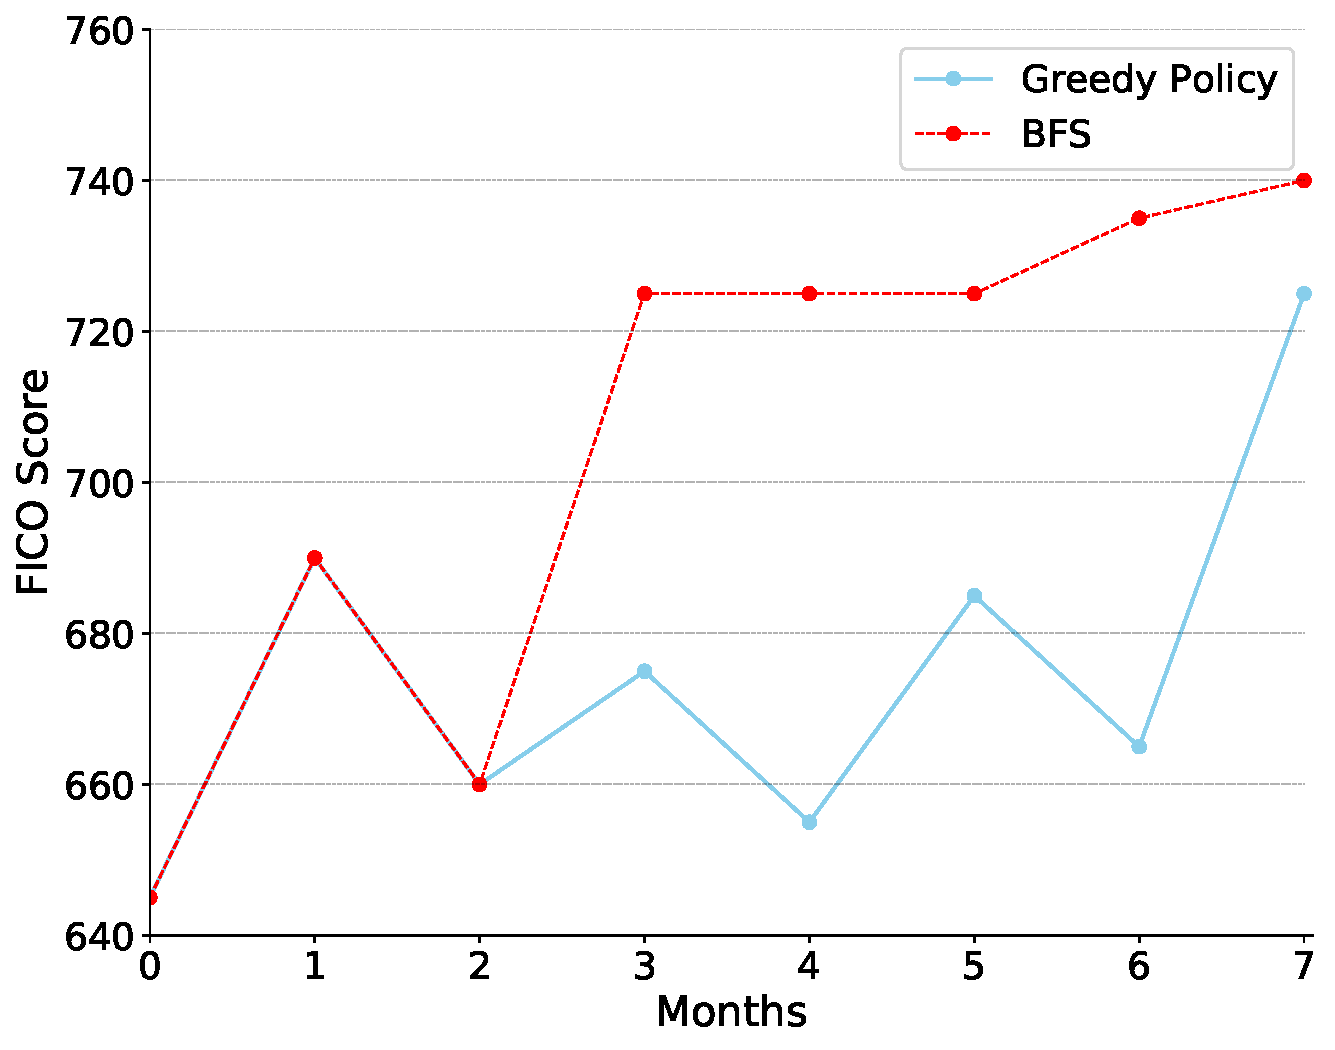
\includegraphics[width=\linewidth]{figures/realfico.pdf}
% \endminipage
    \caption{Comparing the performance of different advice policies, as defined in Eq. \ref{eq:incentivequality}, varying the initial resource count.
    \textbf{Left:} Simple Credit model (averaged over $1000$ initial states, higher is better). \textbf{Center:} recidivism prediction, including race and gender (averaged over $1000$ initially medium/high-risk states, lower is better). \textbf{Right:} Recidivism prediction (excluding race/gender).}
    %(b) Real FICO model. Max score subject to needing \$7500 at the end, given \$10,000 in cash, \$10,000 in debt, 3 cards open (for 2, 7, and 12 months respectively), and no bankrupcies or missed payments.}
    \label{fig:policycomparison}
\end{figure}
\section{Experiments}
\label{sec:experiments}
%\subsection{Decision Settings}
We applied our incentive-evaluation framework to two decision-settings: pretrial risk assessment, and credit scoring. In all cases, we used a discrete action space, and defined $\text{end}(s)$ as whether the agent has expended all their time/changes/resources.

\subheading{Incentive-Approximating Policies}

We compared different incentive-generating policies. To approximate the optimal agency-MDP policy, we used Monte-Carlo Tree Search (\textbf{MCTS}, \cite{browne2012survey}), with random rollouts and $0.5-1$s processing time. For the ``realistic'' credit model (with only 11 actions), we used an exhaustive search of all possible action sequences (\textbf{BFS}).
We also trained a double deep Q-network \cite{van2016deep} on the agency MDP, but found that in both settings the network generally failed to learn a meaningful advice policy (not even equaling the greedy policy), and so we have excluded those results.

We compare these incentives to the \textbf{greedy} policy (Eq. \ref{eq:greedy}), which maximizes the decision immediately after the current action, and to a \textbf{random} policy.


\subheading{Pretrial Risk Assessment Experiment}

In violent pretrial risk assessment, the criminal justice system outputs a score estimating the likelihood of an arrestee to be rearrested for a violent crime within two years, to determine whether to detain the individual pending trial. This offers an interesting case study of incentives, because in addition to accurately preventing violent crimes, the criminal justice system wants to incentivize decision-recipients to avoid criminal activity. We created a pretrial risk-assessment score using ProPublica's COMPAS dataset \cite{angwin_larson_kirchner_mattu_2019}, by training a random forest to use features about the arrestee and the charges from the current arrest to predict $2$-year violent recidivism, and then bucketing the subjects into score groups from 1 (lowest risk) to 10 (highest risk).
% RF params: 200 trees, depth 4, data rebalanced to be 2:1 neg/pos, AUROCs ended up being 
We trained two separate risk scores: one which was blind to the defendant's race and gender (immutable characteristics the subject could not affect), and one which had access to these characteristics. Both scoring algorithms could see a defendant's age - we found that excluding it made any resulting classifier highly inaccurate.

We defined the individual's state as their aforementioned decision features, plus a "number of remaining changes" they could make to their decision features. For a transition model, we allowed the individual, as a single action, to do one of: changing the type of crime (e.g. "drug", "violent", "theft"), incrementing or decrementing the degree of crime (e.g. "1st degree felony", "2nd degree misdemeanor"), or incrementing or decrementing the quantity of a certain type of previous interaction with the justice system (e.g. "\# of prior convictions").

As we can see in Figure \ref{fig:policycomparison}, the agency-MDP-solving policies matched or exceeded the greedy policy in providing agency to individuals across every setting.  Comparing the results between the two recidivism predictors, we see that, on average, excluding race and gender from the model increased individuals' ability to reduce their risk score. This is to be expected: as the decisions can no longer rely on these two immutable characteristics, they rely more heavily on attributes that individuals can hope to affect. 
In Figure \ref{fig:fairrecourse}, we further breakdown the impact of removing race and gender on individuals' agency. We see that the most substantial gains in agency occur among black men, with smaller gains among white men and black women. This provides an interesting counterpoint to conclusions from the fair machine learning literature \cite{dwork2012fairness}: while it may be true that algorithms blind to race or gender may still learn to discriminate based on correlates, blinding the algorithm to immutable characteristics may improve the agency of individuals from disadvantaged populations to change the decisions they receive. This presents an interesting direction for future work.

\begin{figure}
\minipage[t]{0.32\textwidth}
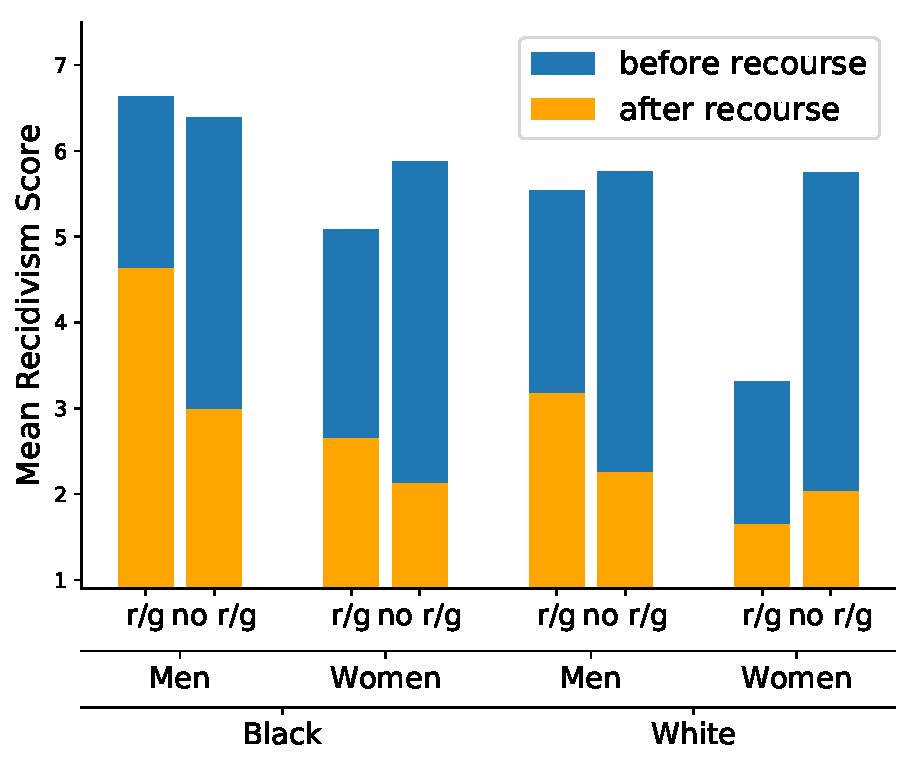
\includegraphics[width=\linewidth]{figures/compas_subgroup-new.pdf}
\caption{Mean recidivism risk score 
%across demographics 
before and after following MCTS-generated incentives for 6 to 10 steps, varying the inclusion of race/gender in decisions.}
    \label{fig:fairrecourse}
\endminipage\hfill
\minipage[t]{0.32\textwidth}
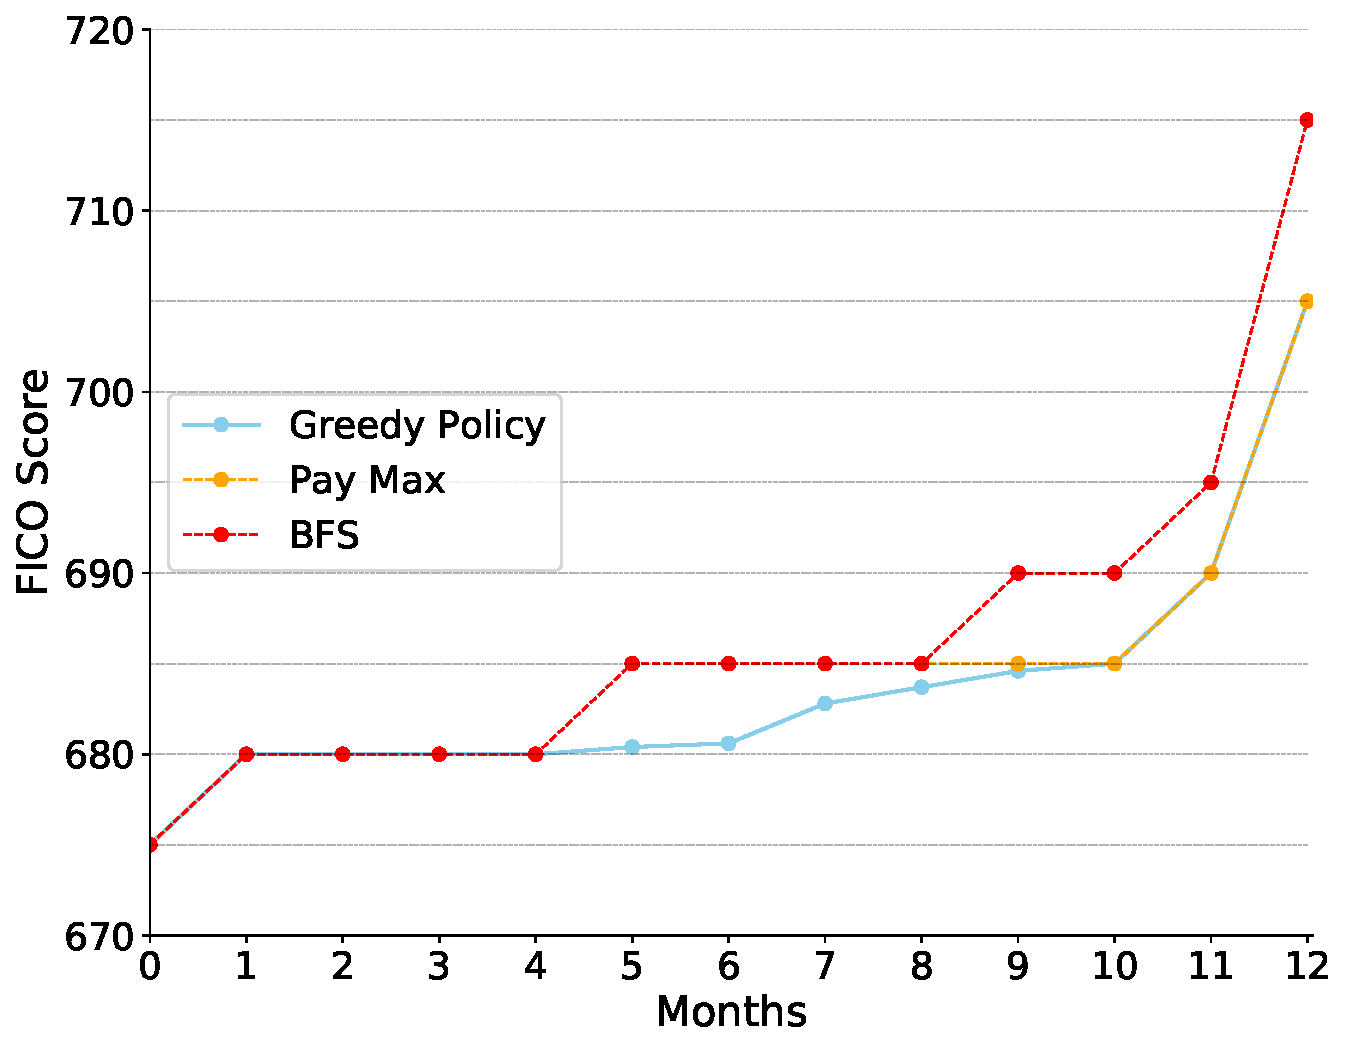
\includegraphics[width=\linewidth]{figures/averageamerican.pdf}
\caption{Credit score under a realistic model, starting with US average financial data and no debt, and varying time remaining before score is checked.}
    \label{fig:averageamerican}
\endminipage\hfill
\minipage[t]{0.32\textwidth}
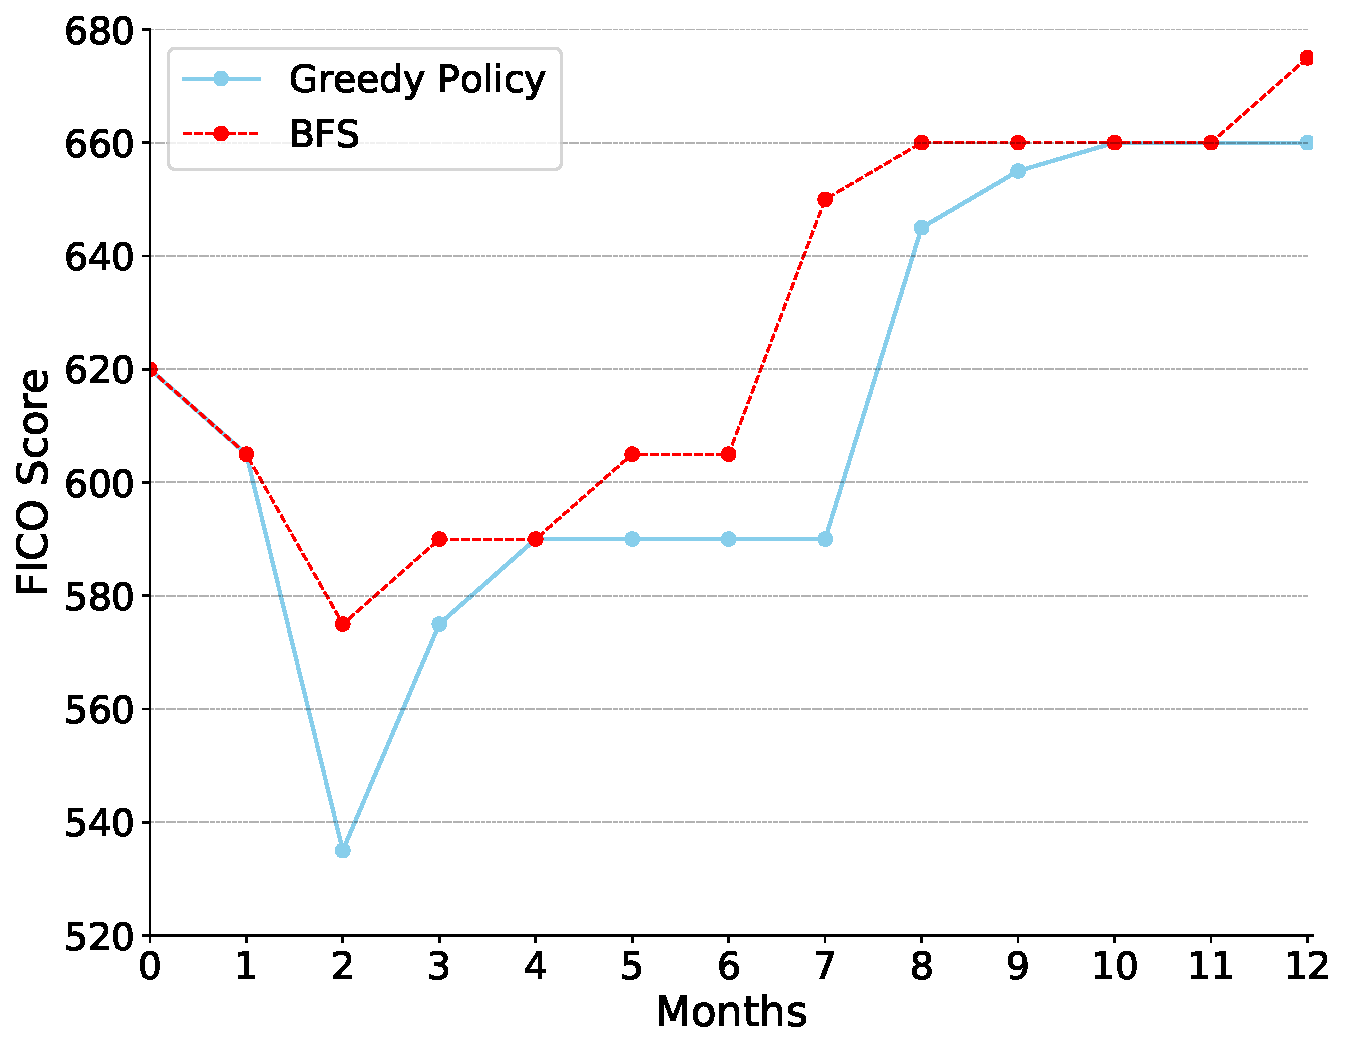
\includegraphics[width=\linewidth]{figures/bankrupt-rand.pdf}
\caption{Credit score under a realistic model, starting with US average financial data but a sudden crisis of \$10,000 of debt, and varying time remaining.}
    \label{fig:bankruptcy}
\endminipage\hfill
\end{figure}

\subheading{Credit Score Experiment}

For credit-scoring, we queried FICO's online credit-estimator \cite{myfico} at $~6\times10^6$ different points, and created a decision-function that output the same decision as the nearest queried point. FICO's estimator used answers to $10$ multiple-answer questions to asses a person's credit. Our "simple" model used these $10$ questions (plus the number of remaining actions) as the state, and allowed any question to be incremented or decremented as an action. We also created a ``realistic'' model (see Figure \ref{fico}), in which the state was comprised of grounded features such as `current cash on hand', `current debt',`how long each card has been open', `last missed payment', and `has declared bankruptcy'. The actions chosen for the transition model were meant to be concrete and achievable (e.g. ``open a credit card and pay the minimum on your cards this month'' rather than ``have less debt''). These actions had sequence-dependent effects like incurring monthly interest on unpaid loans, or declaring bankruptcy (an irreversible action which affected the credit score but simultaneously removed debt).

\begin{figure}
    \centering
\vspace*{-.5cm}
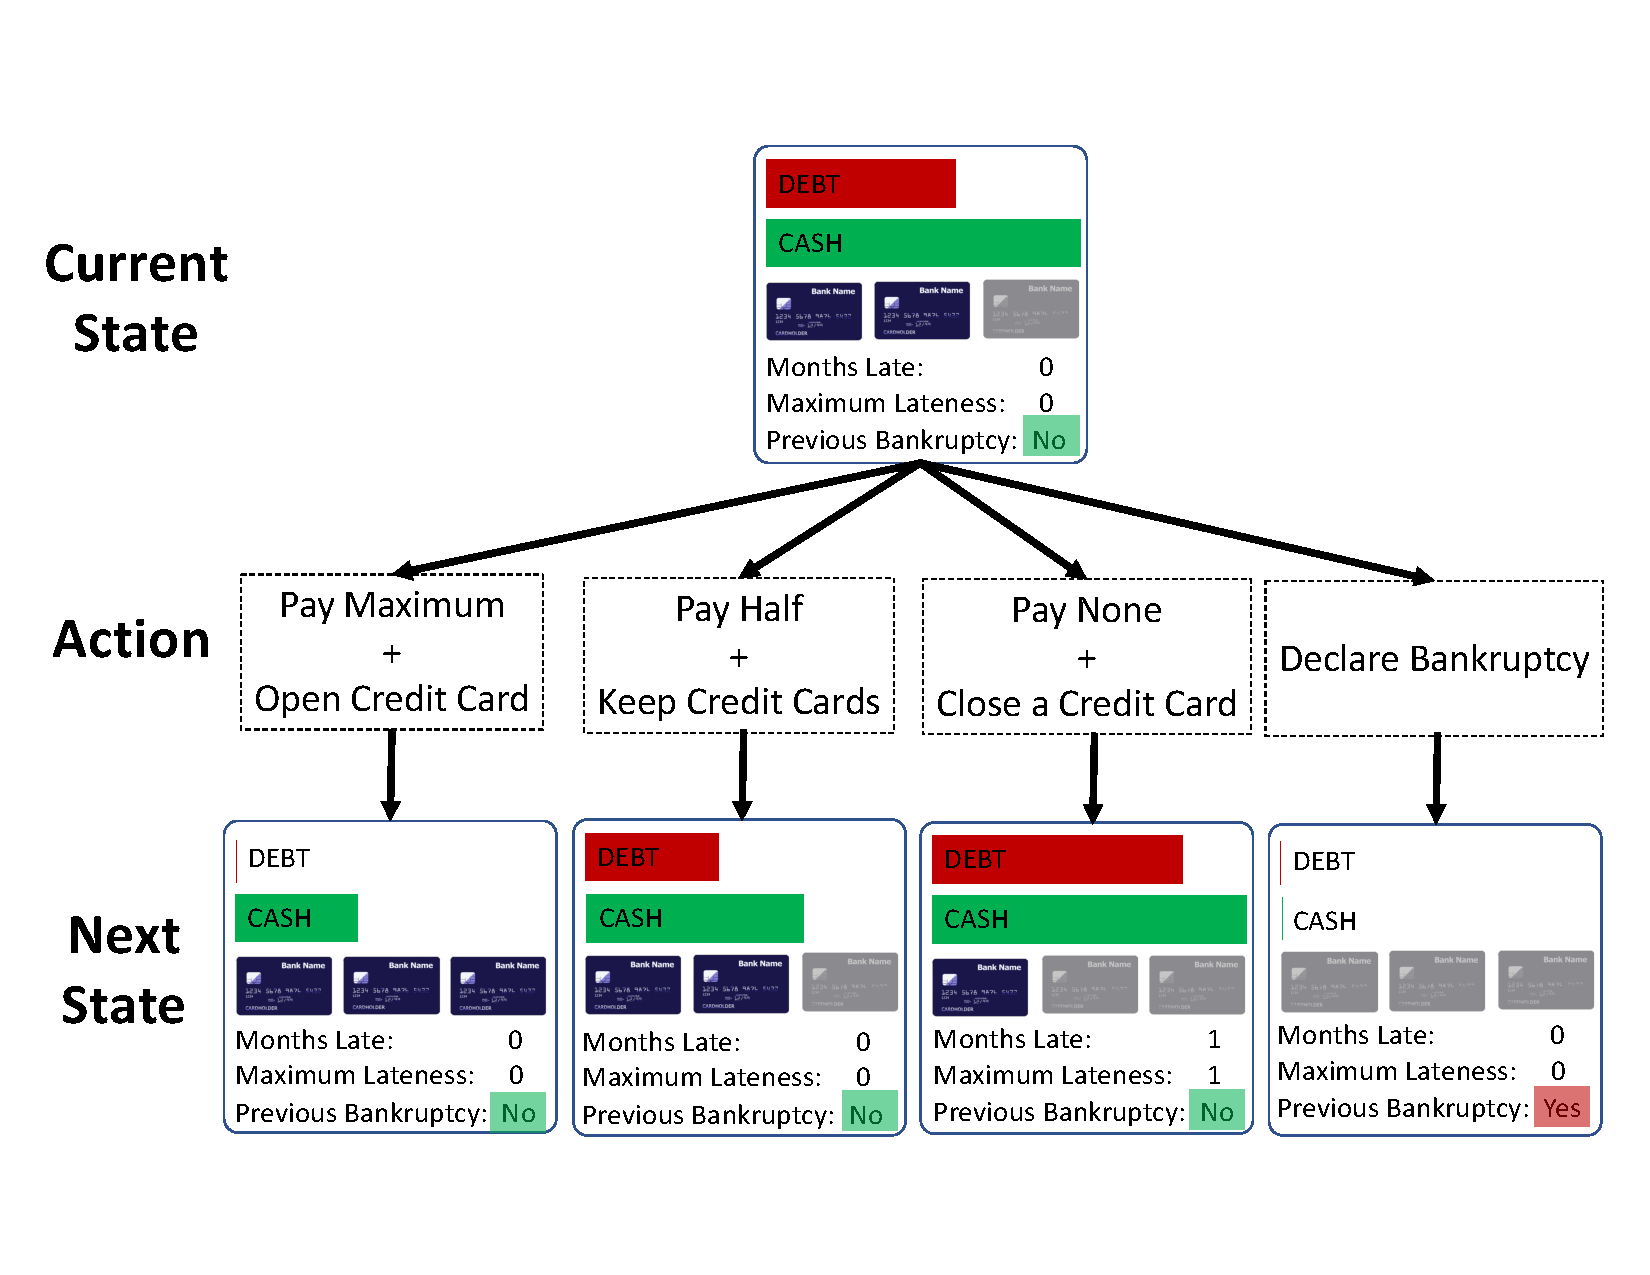
\includegraphics[width=0.5\textwidth, trim=0 60 0 0, clip]
{figures/diagram.pdf}
\caption{Examples of actions an agent can take each month within the ``complex FICO'' model.}
\label{fico}
\vspace*{-.5cm}
\end{figure}

% As seen in Figure \ref{fig:policycomparison}, MDP-based advice policies consistently improved on the greedy policy.
In Figures \ref{fig:averageamerican} and \ref{fig:bankruptcy}, we compared the performance of different advice policies for an average U.S. household (based on income, debt, credit limit, and interest rate) to try to increase their score \cite{frankel_2018,mccann_2019,josephson_josephson_2018}. As we describe below, the greedy policy consistently made short-sighted decisions, while the MDP-solving policy accepted short-term losses for larger long-term gains.

In Figure \ref{fig:averageamerican}, the individual starts off debt-free. The greedy policy always pays the full amount, occasionally opening up a single card in one of the first few months. However, as opening up a second card would decrease the short-term score, the greedy policy only opens a single card. For shorter time-spans, BFS acts similarly to the greedy policy, avoiding opening too many cards to prevent the decrease in credit. 
Given a longer period to act, however, BFS begins by opening up several cards (temporarily decreasing the score), which results in a higher overall score later on. We compared both policies to a ``pay max'' policy that always pays the full amount and doesn't open or close cards. This policy beats greedy on average over the timeframe as greedy doesn't open enough cards to fully reap the benefits of the increased credit limit, and sometimes suffers from the penalty of opening a card.

In Figure \ref{fig:bankruptcy}, the individual starts off with a sudden debt. The greedy policy starts by missing a payment (since the debt doesn't immediately impact the credit score by much), but the interest accrued from this large debt forces the agent to declare bankruptcy in month 2. Given only a month, BFS agrees with the greedy policy and simply misses a payment. However, given more than one month, BFS starts by declaring bankruptcy (knowing it'll happen eventually) so that it can begin rebuilding its credit as quickly as possible.

To highlight the importance of the choice of action-model, we also evaluated what the ``simple'' FICO model, with its simplistic actions, would recommend doing in these "realistic" credit scenarios. For the debt-free scenario, the "simple" BFS advice policy recommended "opening more cards" while keeping fixed the number of recent credit inquiries, and the date the most recent card was opened. While doing so would in fact improve one's credit score, this isn't useful advice, since opening a card without these additional consequences is impossible. For the debt-ridden scenario, the ``simple'' advice policy recommended having less credit card debt -- which, again, is correct but useless advice, since simply "having less debt" is not an executable action.




%%%%% ADD DISCUSSION OF CREDIT SCORE
